
%使用XeLaTeX编译
%版权所有,翻版必究
%本文件由程序自动生成,任何修改将被覆盖
%2019 年 01 月 23 日




\FloatBarrier
\section{
导引
}\label{c000015s000001}


%begin图片
\begin{figure}[htb] %浮动体 here and top ...
%there must use marginnote ...
\marginnote{\setlength\fboxsep{2pt}\fbox{\footnotesize{\kaishu\figurename\,}\footnotesize{\ref{p000012}}}}\centering %中心对齐
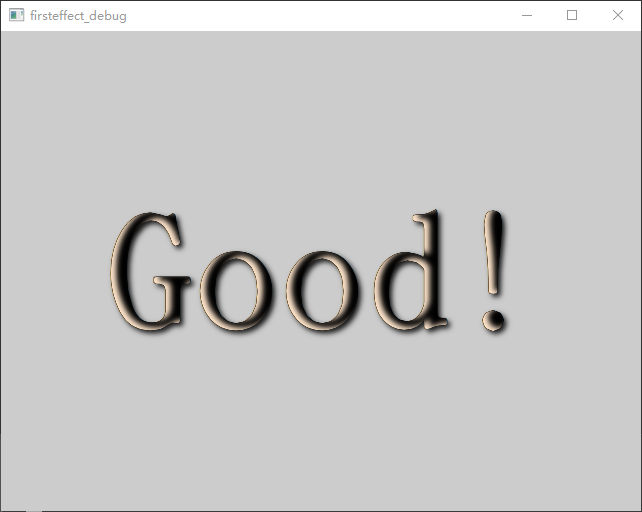
\includegraphics[width=0.95\textwidth]{../chapter06/firsteffect/the_app.png} %图片路径
\caption{文字阴影} %标题
\label{p000012} %索引
\end{figure}
%end图片


tb000000







%使用XeLaTeX编译
%版权所有,翻版必究
%本文件由程序自动生成,任何修改将被覆盖
%2019 年 01 月 23 日



